\documentclass[a4paper,14pt]{extarticle}
\usepackage{geometry}
\usepackage[T1]{fontenc}
\usepackage[utf8]{inputenc}
\usepackage[english,russian]{babel}
\usepackage{amsmath}
\usepackage{amsthm}
\usepackage{amssymb}
\usepackage{fancyhdr}
\usepackage{setspace}
\usepackage{graphicx}
\usepackage{colortbl}
\usepackage{tikz}
\usepackage{pgf}
\usepackage{subcaption}
\usepackage{listings}
\usepackage[colorlinks, linkcolor=blue, urlcolor=blue]{hyperref}
\usepackage{indentfirst}

\usepackage{chngcntr} % нумерация графиков и таблиц по секциям
\counterwithin{table}{section}
\counterwithin{figure}{section}

\graphicspath{{images/}}%путь к рисункам
%\usepackage{mathptmx}

\makeatletter
\renewcommand{\@biblabel}[1]{#1.} % Заменяем библиографию с квадратных скобок на точку:
\makeatother

\geometry{left=2.5cm}% левое поле
\geometry{right=1.5cm}% правое поле
\geometry{top=1.5cm}% верхнее поле
\geometry{bottom=1.5cm}% нижнее поле
\renewcommand{\baselinestretch}{1.5} % междустрочный интервал


\newcommand{\bibref}[3]{\hyperlink{#1}{#2 (#3)}} % biblabel, authors, year
\addto\captionsrussian{\def\refname{Список литературы (или источников)}} 

\renewcommand{\theenumi}{\arabic{enumi}}% Меняем везде перечисления на цифра.цифра
\renewcommand{\labelenumi}{\arabic{enumi}}% Меняем везде перечисления на цифра.цифра
\renewcommand{\theenumii}{.\arabic{enumii}}% Меняем везде перечисления на цифра.цифра
\renewcommand{\labelenumii}{\arabic{enumi}.\arabic{enumii}.}% Меняем везде перечисления на цифра.цифра
\renewcommand{\theenumiii}{.\arabic{enumiii}}% Меняем везде перечисления на цифра.цифра
\renewcommand{\labelenumiii}{\arabic{enumi}.\arabic{enumii}.\arabic{enumiii}.}% Меняем везде перечисления на цифра.цифра

\newcommand{\imgh}[3]{\begin{figure}[h]\center{\includegraphics[width=#1]{#2}}\caption{#3}\label{ris:#2}\end{figure}}

\begin{document}
\begin{titlepage}
\newpage

{\setstretch{1.0}
\begin{center}
Федеральное государственное автономное образовательное учреждение высшего образования «Национальный исследовательский университет «Высшая школа экономики»
\\
\bigskip
Факультет компьютерных наук \\
Основная образовательная программа \\
Прикладная математика и информатика \\
\end{center}
}

\vspace{8em}

\begin{center}
{\Large КУРСОВАЯ РАБОТА}\\
\textsc{\textbf{
Исследовательский проект на тему
\linebreak
"Сжатие словарей для нейросетевого анализа исходных кодов программ"}}
\end{center}

\vspace{2em}

{\setstretch{1.0}
\hfill\parbox{16cm}{
\hspace*{5cm}\hspace*{-5cm}Выполнил студент группы 171, 3 курса,\\
 Гусев Андрей Алексеевич\\
 
\hspace*{5cm}\hspace*{-5cm}Руководитель КР:\\
научный сотрудник Чиркова Надежда Александровна\\

%\hspace*{5cm}\hspace*{-5cm}Куратор:\hfill < степень>, <звание>, <ФИО полностью>\\

\hspace*{5cm}\hspace*{-5cm}Консультант:\\
научный сотрудник Лобачева Екатерина Максимовна\\
}
}

\vspace{\fill}

\begin{center}
Москва 2020
\end{center}

\end{titlepage}% это титульный лист
\newpage

{
	\hypersetup{linkcolor=black}
	\tableofcontents
}

\newpage

\section{Введение} 
\subsection{Описание предметной области}

Пример, как использовать ссылки на источник:\\
В качестве базовой модели для тестирования разработанного алгоритма была взята модель \bibref{code2seq}{Alon et al.}{2019}.

График \ref{fig:by_epochs} достаточно бессмысленный без контекста.

\begin{figure}[h!]
	\centering
	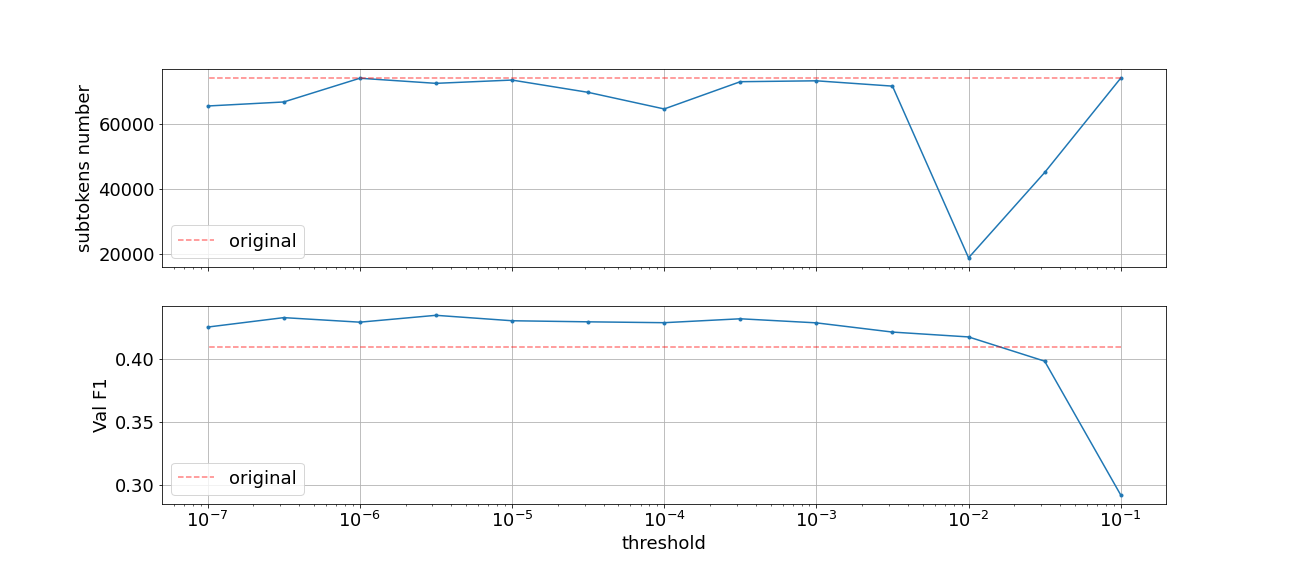
\includegraphics[width=1\textwidth]{graphics/example.png}
	\caption{Графики зависимостей разреженностей и качества от числа эпох }
	\label{fig:by_epochs}
\end{figure}



\begin{thebibliography}{0}
\bibitem{codenn}\hypertarget{codenn}{}
\href{https://www.aclweb.org/anthology/P16-1195.pdf}
{Srinivasan Iyer, Ioannis Konstas, Alvin Cheung, Luke Zettlemoyer. Summarizing Source Code using a Neural Attention Model. In ACL 2016.}
\bibitem{chirkova18}\hypertarget{chirkova18}{}
\href{https://arxiv.org/abs/1810.10927}
{Nadezhda Chirkova, Ekaterina Lobacheva, Dmitry Vetrov. Bayesian Compression for Natural Language Processing. In EMNLP 2018.}
\bibitem{code2seq}\hypertarget{code2seq}{}
\href{https://openreview.net/pdf?id=H1gKYo09tX}
{Uri Alon, Shaked Brody, Omer Levy, Eran Yahav. Code2Seq: Generating sequences from structured representations of code. In ICLR 2019.}
\end{thebibliography}


\end{document}

